\subsection{PostgreSQL Configuration}\label{subsec:postgresql-configuration}
\begin{flushleft}
    Currently, the database contains 2 databases.
    \begin{itemize}
        \item contact\_form
        \item shop
    \end{itemize}
    As a security feature, the login either by local or remote host, have enabled "SCRAM-SHA-256".
\end{flushleft}
\subsubsection[Contact database]{Contact database}
\begin{flushleft}
    As the name hints, this database is used to store the contact forms received using the contact page from the website.
    Yet, the database consists of one table.
\end{flushleft}

\begin{center}
    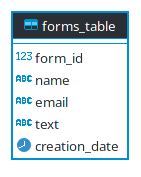
\includegraphics[scale=0.6]{DB_Table_Schema_Contact_FormV1}
\end{center}
\begin{center}
    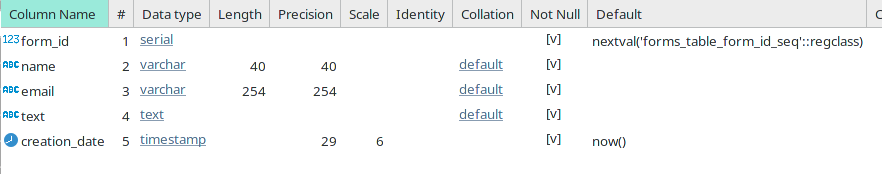
\includegraphics[scale=0.6]{DB_Table_Table_Contact_Form}
\end{center}

\begin{flushleft}
    As the name hints, this database is used to store the contact forms received using the contact page from the website.
    Yet, the database consists of one table.
\end{flushleft}
\begin{flushleft}
    It also contains a procedure called "insert\_form", which given the next information \"\textit{(p\_name varchar,
    p\_email varchar, p\_text text)}", checks if the values are valid and in case of not being valid, will rise an error
    (more information in the REGEX and Error threads).

\end{flushleft}